\documentclass[a4paper]{article}

\usepackage[dvipsnames]{xcolor}
\usepackage[T1]{fontenc}
\usepackage[utf8]{inputenc}
\usepackage{lmodern}

\usepackage[english]{babel}
\usepackage{csquotes}

\usepackage{graphicx}
\graphicspath{ {./images/} }

\usepackage[margin=0.6in]{geometry}

\usepackage[notes,backend=biber]{biblatex-chicago}
\bibliography{sample}

\begin{document}
\title{Unsupervised Learning - CS 4641}
\author{Omar Shaikh}
\maketitle

\begin{abstract}
    In this report, I covered two fundamental unsupervised machine learning algorithms: K-means and Gaussian Mixture Models. To do this, I selected two different data-sets -- images of histopathologic-cancer tumors and the classic Iris Flower Dataset. First, I introduced each data-set and our unsupervised classification problem; then, I ran the clustering algorithms on the datasets and described my results, both before and after running the aforementioned dimensionality reduction algorithms. 
    
    The next section involved neural network analysis on a single dataset. For this option, I picked the Iris dataset. First, I reran my neural network learner on only the dimension reduced datasets and discussed my results. Then, I treated the clustering algorithms as dimensionality reduction algorithms, running my neural network learner on this newly projected data. In the comparative analysis section, I tested each algorithm on the withheld testing data, showcasing the strengths and weaknesses of each while answering some questions.
\end{abstract}

\section{Dataset \& Classification Problems}
\subsection{PCam Dataset \& Classification}

The first dataset I used (same as assignment \#1) is the CAMELYON dataset, collected by Department of Pathology of the Radboud University Medical Center (Radboudumc) in Nijmegen, The Netherlands \autocite{doi:10.1093/gigascience/giy065}. I found this dataset after searching for labelled cancer images datasets.

The dataset has binary labels: either the cells have metastasized (1 label), or they have not (0 label). For the sake of speed, I chose to undersample this dataset such that N=88010, instead of N=220025. The undersampled dataset has a 60-40 split. See figure 1 for a breakdown of the undersampled dataset. 

Finally, why this dataset? My family has an unfortunate genetic history with cancer, so a related project was generally of interest. Also, computer vision is considered a strength of deep neural networks -- working with an image based dataset would help me see if and why this is so.

\subsubsection{General Feature Engineering}
Although images provided were a 96x96 slide, only the center 32x32 contained tumor tissue. For classifiers used in this report, I cropped the images and converted them to black and white beforehand. I also rescaled the data to have zero mean and one standard deviation. 

\begin{figure}
  \centering
  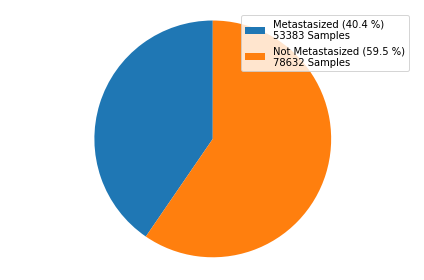
\includegraphics[width=0.4\textwidth]{images/pcamDistr.png}
  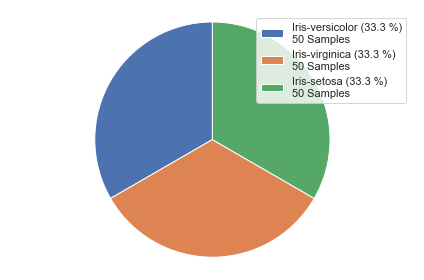
\includegraphics[width=0.4\textwidth]{images/irisDistr.png}
  \caption{Breakdown of the datasets; Undersampled PCam (left), Iris (right)}
\end{figure}

\subsection{Iris Flower Dataset}

I found this dataset on Kaggle after searching for risk analytics challenges; it was collected during the a research collaboration between Worldline and the Machine Learning Group of ULB (Université Libre de Bruxelles) \autocite{dal2015calibrating}. This dataset poses a unique to me because it's highly imbalanced -- there are only a few (proportionally) samples of fradulent credit cards. Also, the actual credit card data (28 features, aside from the date and amount) were anonymized with PCA analysis; working with a dataset without having access to the original information itself was a unique challenge

A short except from the Kaggle challenge, along with figure 1, highlights the breakdown of the dataset:

\begin{quote}
The datasets contains transactions made by credit cards in September 2013 by European cardholders. This dataset presents transactions that occurred in two days, where we have 492 frauds out of 284,807 transactions [also a binary classification task]. The dataset is highly unbalanced, the positive class (frauds) account for 0.172 \% of all transactions \autocite{Kaggle-CreditCard}.
\end{quote}

Finally, why this dataset? I couldn't use my old dataset from Assignment 1 because the data already underwent dimensionality reduction. I wanted to find a dataset that was easily visualized after projections so that viewing the clusters would be easy for analysis.

\subsubsection{Feature Engineering and Modified Model Assessment}
Before worrying about oversampling, I normalized the the date and amount values to lie within the same range as the PCA anonymized credit card data. Then, to deal with over-representation of one of the classes (transaction detected as a fraud), I needed to find a method to represent and evaluate the features in my dataset. Training the model would require us to under-sample the dataset, such that X and Y would have equal proportions of fraudulent and non-fraudulent datsets. 

The dataset was initially split into an original\_X\_test and original\_Y\_test -- this is a 90-10 split. Then, I generated an under-sampled dataset from all the 492 fraud instances. On this secondary under-sampled dataset, I split again with 80-20, creating a training and testing dataset. This is training set I ran cross validation on in the algorithm subsections. Finally, in the comparative analysis, I evaluated the under-sampled 20\% alongside the entire with-held 10\% with the ROC-AUC score.

Note that for the testing of this dataset, I would test two separate sets in comparative analysis: the entire dataset, and the withheld 20\% from the under-sampled subset. Because of severe overrepresentation problems, I will use the Area Under the Receiver Operating Characteristic Curve (ROC AUC) for the comparative analysis testing, instead of accuracy during model training.

\subsection{Exploring PCam}
\subsubsection{Clustering}
\subsubsection{Dimensionality Reduction}
\subsection{Exploring Iris}
\subsubsection{Clustering}
\subsubsection{Dimensionality Reduction}
\subsection{Comparative Analysis I}
\subsection{Neural Networks with Iris}
\subsubsection{Testing NNs on Dimensonality Reduced Data}
\subsubsection{Testing NNs on Cluster Reduced Data}
\subsection{Comparative Analysis II} 
\printbibliography

\end{document}